\documentclass[border=10pt]{standalone}
\usepackage[svgnames]{xcolor}
\usepackage{amsmath}
\usepackage{pgfplots}
\pgfplotsset{compat=newest}
\usepackage[sfdefault]{FiraSans}
\usepackage{FiraMono}
\renewcommand*\familydefault{\sfdefault}
\begin{document}
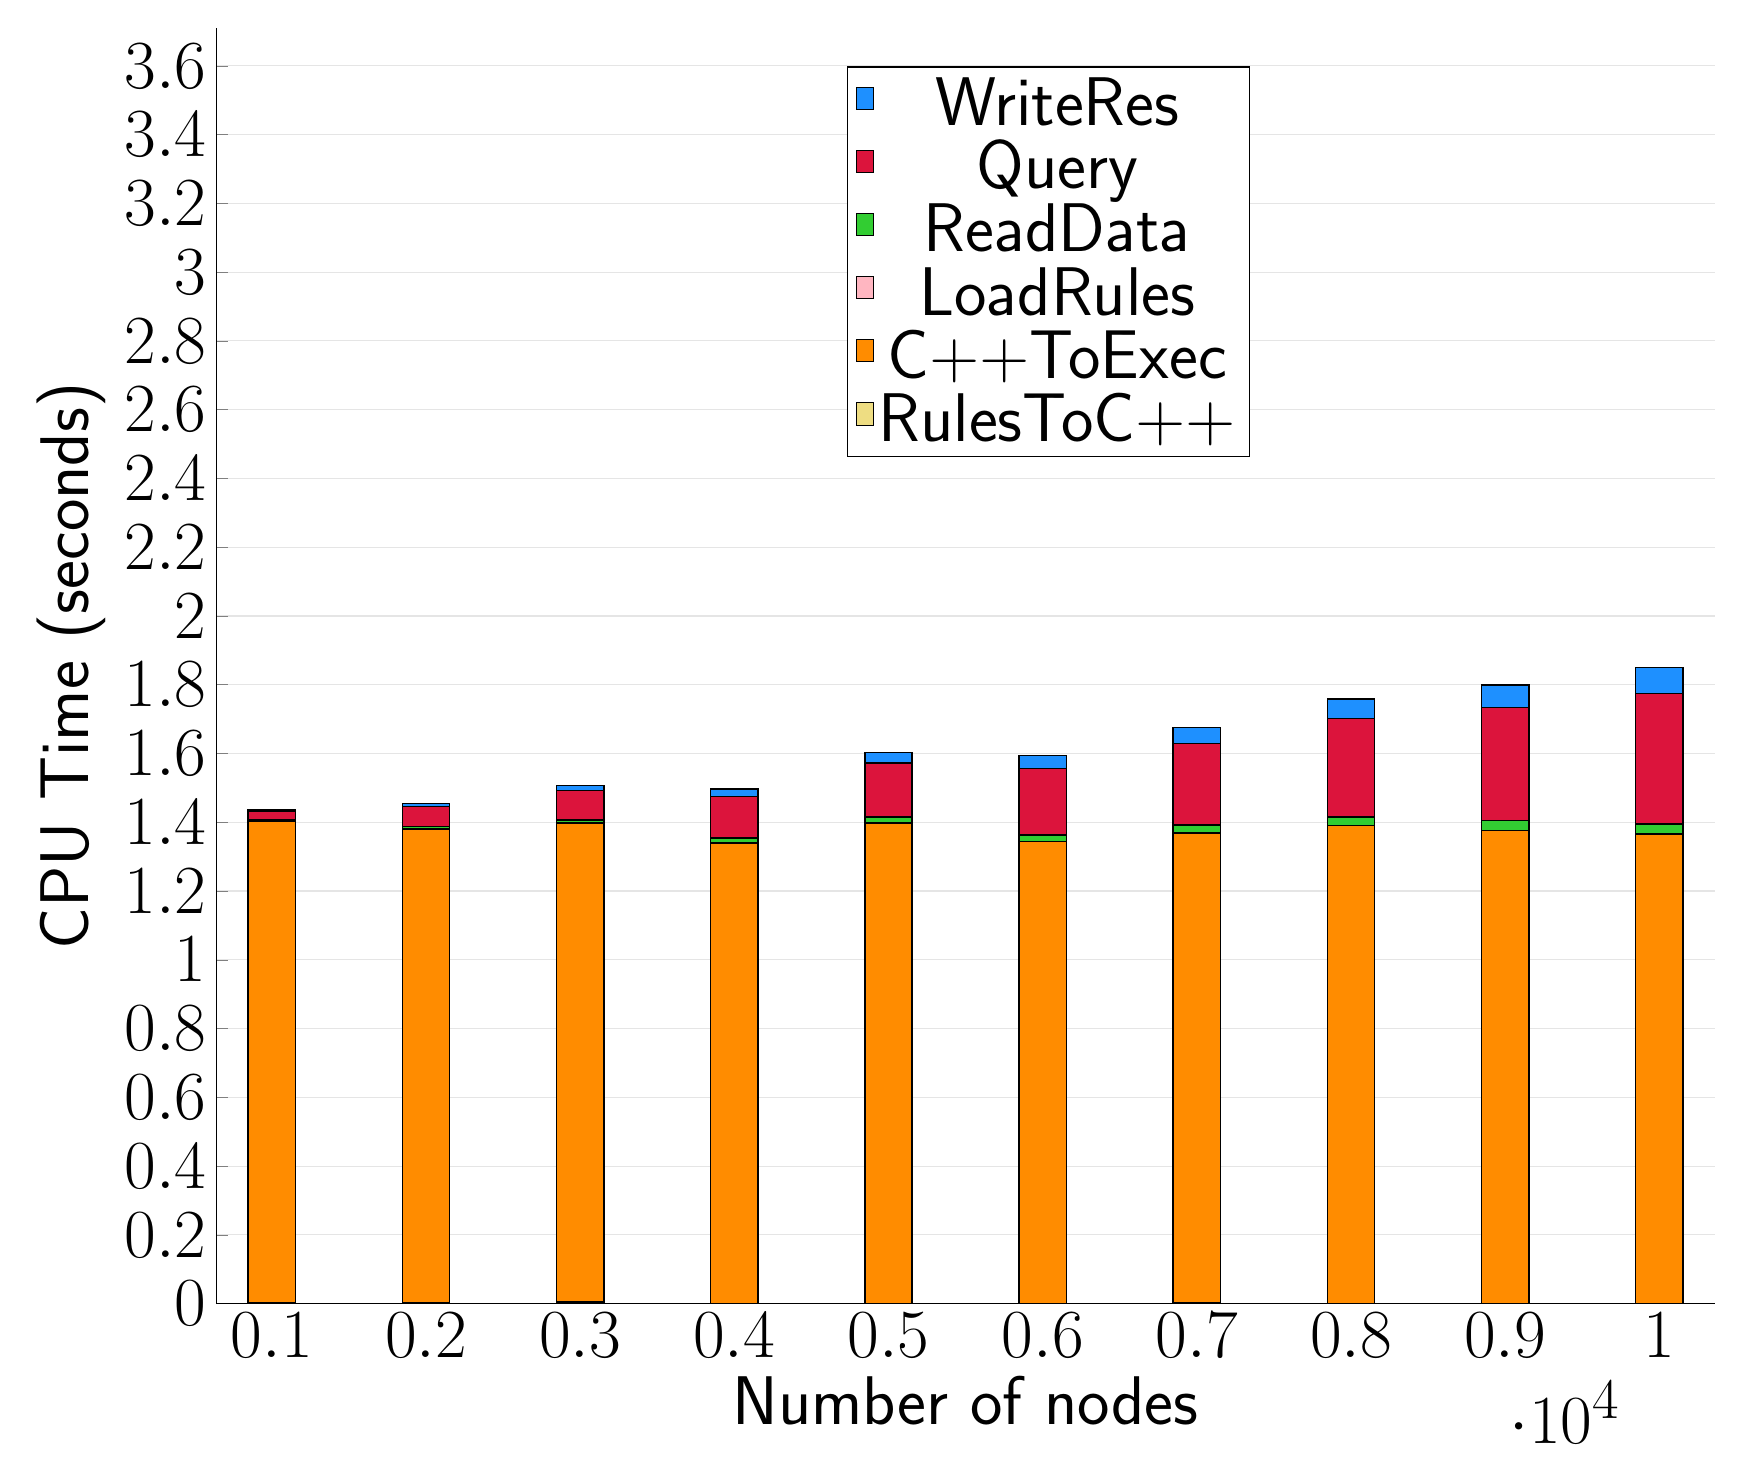
\begin{tikzpicture}
\begin{axis}[
   ybar stacked,
   width=1.7\textwidth,
   bar width=0.6cm,
   ymajorgrids, tick align=inside,
   major grid style={draw=gray!20},
   xtick=data,
   ymin=0, ymax=3.70944,
   axis x line*=bottom,
   axis y line*=left,
   enlarge x limits=0.04,
   legend style={
       at={(0.69, 0.97)},
       anchor=north east,
       legend columns=1,
       font=\Huge,
   },
   ylabel={CPU Time (seconds)},
   xlabel={Number of nodes},
   label style={font=\Huge},
   tick label style={font=\Huge},
]
\addlegendimage{fill=DodgerBlue, draw=black, line width=0.2pt}
\addlegendentry{WriteRes}
\addlegendimage{fill=Crimson, draw=black, line width=0.2pt}
\addlegendentry{Query}
\addlegendimage{fill=LimeGreen, draw=black, line width=0.2pt}
\addlegendentry{ReadData}
\addlegendimage{fill=LightPink, draw=black, line width=0.2pt}
\addlegendentry{LoadRules}
\addlegendimage{fill=DarkOrange, draw=black, line width=0.2pt}
\addlegendentry{C++ToExec}
\addlegendimage{fill=LightGoldenrod, draw=black, line width=0.2pt}
\addlegendentry{RulesToC++}
\addplot +[fill=LightGoldenrod, draw=black, line width=0.55pt] coordinates {
(1000, 0.0020000000000000018)
(2000, 0.001999999999999999)
(3000, 0.0040000000000000036)
(4000, 0.0)
(5000, 0.0)
(6000, 0.0)
(7000, 0.0020000000000000018)
(8000, 0.0)
(9000, 0.0)
(10000, 0.0)
};
\addplot +[fill=DarkOrange, draw=black, line width=0.55pt] coordinates {
(1000, 1.4000000000000001)
(2000, 1.3780000000000001)
(3000, 1.3940000000000001)
(4000, 1.3400000000000003)
(5000, 1.3980000000000001)
(6000, 1.344)
(7000, 1.366)
(8000, 1.3900000000000001)
(9000, 1.3760000000000001)
(10000, 1.366)
};
\addplot +[fill=LightPink, draw=black, line width=0.55pt] coordinates {
(1000, 0.0001308)
(2000, 0.00014739999999999998)
(3000, 0.0001174)
(4000, 0.0001574)
(5000, 0.00015160000000000003)
(6000, 0.00012139999999999998)
(7000, 0.00015279999999999997)
(8000, 0.0001426)
(9000, 0.00016460000000000002)
(10000, 0.0001242)
};
\addplot +[fill=LimeGreen, draw=black, line width=0.55pt] coordinates {
(1000, 0.003881)
(2000, 0.007964599999999999)
(3000, 0.008616200000000001)
(4000, 0.014333599999999998)
(5000, 0.0166736)
(6000, 0.0188528)
(7000, 0.0243738)
(8000, 0.0249954)
(9000, 0.028394799999999998)
(10000, 0.0289084)
};
\addplot +[fill=Crimson, draw=black, line width=0.55pt] coordinates {
(1000, 0.024625599999999997)
(2000, 0.0577718)
(3000, 0.0850326)
(4000, 0.12063540000000002)
(5000, 0.1578734)
(6000, 0.1932738)
(7000, 0.2363998)
(8000, 0.2866352)
(9000, 0.32940200000000003)
(10000, 0.37972)
};
\addplot +[fill=DodgerBlue, draw=black, line width=0.55pt] coordinates {
(1000, 0.0043426)
(2000, 0.009072)
(3000, 0.0149316)
(4000, 0.0220078)
(5000, 0.029977999999999998)
(6000, 0.0378284)
(7000, 0.0467188)
(8000, 0.056391000000000004)
(9000, 0.0655744)
(10000, 0.0754248)
};
\end{axis}
\end{tikzpicture}

\end{document}
